\documentclass[12pt]{article}
\usepackage{amsmath}
\usepackage{mathtools}
\usepackage{bigints}
\usepackage{parskip}
\usepackage{amssymb}
\usepackage{relsize}
\usepackage{fullpage}
% \DeclareMathSizes{12}{17.28}{9}{7} % (a)

\DeclareMathSizes{12}{17.28}{12}{12} % (a)


\usepackage{hyperref}



	\addtolength{\topmargin}{-.5in}
	\addtolength{\textheight}{1.75in}



    \newenvironment{myindentpar}[1]%
     {\begin{list}{}%
             {\setlength{\leftmargin}{#1}}%
             \item[]%
     }
     {\end{list}}

\begin{document}
\title{College Algebra: Module 9 What You Need To Know}
\date{3-22-15}
\author{}
\maketitle


\section{Piecewise Defined Functions (Section 3.4)}

\textbf{Piecewise Function} - a \textit{piecewise function} is a function that is a combination of two or more sub-functions where each sub-function is defined over its own unique interval. Below is an example of a piecewise function:
\newline

\centerline{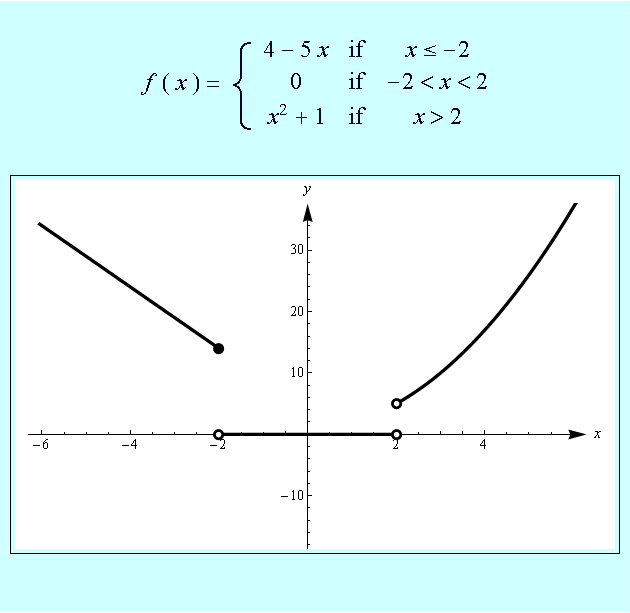
\includegraphics{PiecewiseFunction.png}}

\newpage

\textbf{Evaluating Piecewise Functions}

Consider the same piecewise function that was given on the first page of the notes:

 \begin{displaymath}
   f(x) = \left\{
     \begin{array}{lr}
       4-5x & x \leq -2\\
       0 & -2 < x < 2\\
      x^2 + 1 &   x > 2
     \end{array}
   \right.
\end{displaymath} 

 Let's try find the values $f(-4), f(-2), f(0), f(2),\text{ and } f(3)$. 

$f(-4) = 4 - 5(-4) = 4+ 20 = 24$ 

$f(-2) = 4-5(-2) = 4+10 = 14$ 

$f(0) = 0$ 

$f(2)$ is undefined 

$f(3) = 3^2 + 1 = 10$ 


\section{The Algebra and Composition of Functions (Section 3.5)}

\textbf{Sum, Difference, Product, and Quotient of Functions:}

Let $f(x)$ and $g(x)$ be any two functions. We can find the sum, difference, product, and quotient of them as given by the following rules:
\begin{enumerate}

\item \textbf{Sum:} $(f + g)(x) = f(x) + g(x)$
\item \textbf{Difference:} $(f - g)(x) = f(x) - g(x)$
\item \textbf{Product:} $(f  \cdot g)(x) = f(x) \cdot g(x)$
\item \textbf{Quotient:} $\dfrac{f}{g}(x) = \dfrac{f(x)}{g(x)}$

\end{enumerate}

\textbf{Function Composition:} 

$(f \circ g)(x) = f \Big(g(x)\Big)$
\begin{myindentpar}{1cm}


\textbf{Example:} Let $f(x) = 3x^2-2$ and $g(x) = \dfrac{x+2}{x-1}$ 

Then $f \circ g = 3 \Big(\dfrac{x+2}{x-1} \Big)^2 -2$

\textbf{Note:} BE CAREFUL when finding the domain of a composition of functions. 
\end{myindentpar}
\begin{myindentpar}{2cm}
\textbf{Example:} Let $f(x) = \sqrt{x-12}$ and $g(x) = x^2-4$

Find 

a) $f \circ g$ 

b) $g \circ f$ 

and state the domain of each
\end{myindentpar}
\begin{myindentpar}{2.5cm}
\textbf{Answer:}
 \textbf{a)} $f \circ g = \sqrt{(x^2-4)-12}$

\hspace{3.3cm} $ = \sqrt{x^2-16}$

\textbf{Domain:} $x^2 - 16 \geq 0 \implies x\leq -4$ and $x \geq 4$

So the domain in interval notation is $(-\infty, -4] \cup [4, \infty)$

\textbf{Answer: b)} $g \circ f = \Big(\sqrt{x-12}\Big)^2 -4$

\hspace{3.3cm} $ = x-12 -4$

\hspace{3.3cm} $ = x-16$

\textbf{Domain:} $x - 12 \geq 0 \implies x \geq  12 \implies [12 , \infty)$
\end{myindentpar}


\section{Quadratic Functions and Applications (Section 4.1)}

\textbf{Standard Form of a Quadratic Function} 
\newline

\centerline{$f(x) = ax^{2} + bx  + c$}

\hspace{6cm} $a > 0 \to$ Upward Pointing

\hspace{6cm} $a < 0 \to$ Downward Pointing

\textbf{Vertex Form of a Quadratic Function:}
\newline

\centerline{$f(x) = a(x-h)^{2} + k$}

\hspace{6.5cm} Vertex: $(h,k)$

\hspace{6.5cm} $a > 0 \to$ Upward Pointing

\hspace{6.5cm} $a < 0 \to$ Downward Pointing

\textbf{Vertex of a Parabola:}
\newline

\centerline{$\Big(-\dfrac{b}{2a}, f(-\dfrac{b}{2a}) \Big)$}

\vspace{1cm}

\textbf{Converting Between Standard Form and Vertex Form:} COMPLETE THE SQUARE

\textbf{Example:} Write $2x^2 + 8x + 7$ in vertex form and identify the vertex

\begin{enumerate}

\item Group first two terms: $(2x^2 + 8x) + 7$
\item Factor out $a$ from the first two terms: $2(x^2 + 4x) + 7$
\item Compute $\Big(\dfrac{b}{2a}\Big)^2$ and add and subtract this inside: $2(x^2 + 4x + 4  - 4) + 7$
\item Factor: $2\Big((x+2)^2 - 4\Big) + 7$
\item Distribute $a$ back inside: $2(x+2)^2 - 8 + 7$
\item Combine the constant terms: $2(x+2)^2 - 1$

\end{enumerate}

This is now in vertex form. The vertex is $(-2,-1)$

\textbf{Finding the X-Intercepts of a Quadratic} - Set $y = 0$ and solve for $x$ either by factoring, completing the square, or using the quadratic formula

\textbf{Finding the Maximum/Mininum of a Quadratic $ax^2 + bx + c$}

$a > 0 \to $ parabola is upward pointing so there is no maximum, but there is a minimum. The minimum is the y-value of the vertex. If you can find the vertex, then you will find the minimum value.

$a < 0 \to $ parabola is downward pointing so there is no minimum, but there is a maximum. The maximum is the y-value of the vertex. If you can find the vertex, then you will find the maximum value.

Problem 1: Find all entire functions $f$ such that $\int\int |f(x+iy)|^2dxdy<\infty$.

Problem 2: If $\mathbb{D}$ is the open unit disk and $f: \mathbb{D} \to  \overline{\mathbb{D}}$ is an analytic function then show that $|f^{(n)}(z)|\leq n!(1-|z|)^n$, for all $z\in \mathbb D$.















































\end{document}